\subsection{Kennzahlen}
    Auch in diesem Fallbeispiel wurde eine Reihe an Kennzahlen ermittelt,
    die in diesem Kapitel präsentiert werden.

    \paragraph{Struktur eines Graphen}
    Zum Verständnis der Zahlen trägt Abbildung \ref{image:findingNewsFiguresDbModel} bei,
    welche den Aufbau des Graphen visualisiert.
    Wegen der beschriebenen Überschneidung mit dem ersten Fallbeispiel,
    sind die übereinstimmenden Knoten hier nicht nochmals dargestellt.
    Wie im vorherigen Beispiel wird außerdem auf die Darstellung von
    Referenzen verzichtet.

    \begin{figure}[htb]
        \centering
        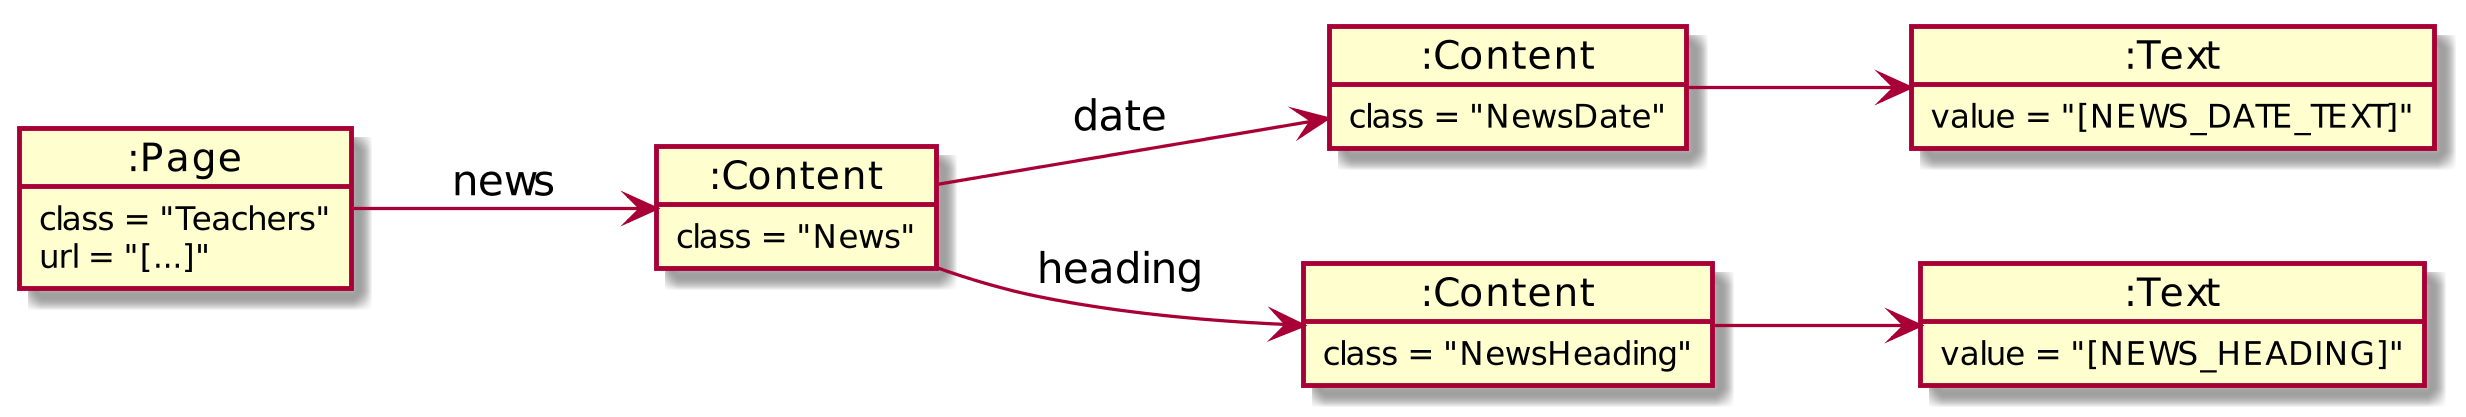
\includegraphics[scale=\imageScalingFactor]{../resources/findings/case-study-2/dbmodel.png}
        \caption{Struktur des Graphen einer Seite über aktuelle Meldungen}
        \label{image:findingNewsFiguresDbModel}
    \end{figure}

    \paragraph{Präsentation der Kennzahlen}
    Die folgenden Tabellen präsentieren die gesammelten Kennzahlen.
    Die Gruppierung der Knoten nach ihren Labels ist in Tabelle
    \ref{table:findingsNewsFiguresNodesByLabel} zu sehen.
    Die Häufigkeit der Inhaltsklassen stellt Tabelle
    \ref{table:findingsNewsFiguresContentNodesByClass} dar.
    Tabelle \ref{table:findingNewsFiguresEdgesByLabel} gruppiert die Kanten der Datenbank
    nach ihren Labels und Tabelle
    \ref{table:findingsNewsFiguresEdgesByStartEndNodeLabel}
    stellt heraus, welche Knotenarten diese Kanten verbinden.
    Zuletzt betrachtet Tabelle \ref{table:findingsNewsFiguresSharedNodes}
    die Frage, welche Knoten mehrfach referenziert wurden.

    \begin{table}[htb]
        \begin{subtable}[c]{0.3\textwidth}
            \centering
            \begin{tabular}{|l|c|}
                \hline
                \textbf{Label}  & \multicolumn{1}{l|}{\textbf{Anzahl}} \\ \hline
                \texttt{Content}         & 124                                  \\ \hline
                \texttt{Page} + \texttt{Resource} & 5                                    \\ \hline
                \texttt{Resource}        & 53                                   \\ \hline
                \texttt{Site}            & 1                                    \\ \hline
                \texttt{Text}            & 77                                   \\ \hline
                \hline
                \textbf{Summe}  & 260                                  \\ \hline
            \end{tabular}
            \subcaption{Knoten gruppiert nach Labels für Seiten über aktuelle Meldungen}
            \label{table:findingsNewsFiguresNodesByLabel}
        \end{subtable}
        \begin{subtable}[c]{0.3\textwidth}
            \centering
            \begin{tabular}{|l|c|}
                \hline
                \textbf{Klasse} & \multicolumn{1}{l|}{\textbf{Anzahl}} \\ \hline
                \texttt{Brand}           & 1                                    \\ \hline
                \texttt{Header}          & 1                                    \\ \hline
                \texttt{News}            & 41                                   \\ \hline
                \texttt{NewsDate}        & 38                                   \\ \hline
                \texttt{NewsHeading}     & 41                                   \\ \hline
                \texttt{PageHeading}     & 1                                    \\ \hline
                \texttt{Portal}          & 1                                    \\ \hline
                \hline
                \textbf{Summe}  & 260                                  \\ \hline
            \end{tabular}
            \subcaption{\texttt{Content}-Knoten gruppiert nach ihrer Klasse für Seiten über aktuelle Meldungen}
            \label{table:findingsNewsFiguresContentNodesByClass}
        \end{subtable}
        \begin{subtable}[c]{0.3\textwidth}
            \centering
            \begin{tabular}{|l|c|}
                \hline
                \textbf{Label} & \multicolumn{1}{l|}{\textbf{Anzahl}} \\ \hline
                \texttt{Reads}          & 80                                   \\ \hline
                \texttt{References}     & 87                                   \\ \hline
                \texttt{Owns}           & 145                                  \\ \hline
                \hline
                \textbf{Summe} & 312                                  \\ \hline
                \end{tabular}
            \subcaption{Kanten gruppiert nach Labels für Seiten über aktuelle Meldungen}
            \label{table:findingNewsFiguresEdgesByLabel}
        \end{subtable}

        \begin{subtable}[c]{0.5\textwidth}
            \centering
            \begin{tabular}{|l|c|}
                \hline
                \textbf{Start $\rightarrow$ Ziel} & \multicolumn{1}{l|}{\textbf{Anzahl}} \\ \hline
                \texttt{(:Content)} $\rightarrow$ \texttt{(:Content)}     & 83                                   \\ \hline
                \texttt{(:Content)} $\rightarrow$ \texttt{(:Resource)}    & 49                                   \\ \hline
                \texttt{(:Page)} $\rightarrow$ \texttt{(:Content)}        & 57                                   \\ \hline
                \texttt{(:Page)} $\rightarrow$ \texttt{(:Page)}           & 13                                   \\ \hline
                \texttt{(:Page)} $\rightarrow$ \texttt{(:Resource)}       & 25                                   \\ \hline
                \texttt{(:Site)} $\rightarrow$ \texttt{(:Page)}           & 5                                    \\ \hline
                \textbf{Summe}                    & 232                                  \\ \hline
            \end{tabular}
            \subcaption{Kanten gruppiert nach Labels der Start- und Zielknoten für Seiten über aktuelle Meldungen}
            \label{table:findingsNewsFiguresEdgesByStartEndNodeLabel}
        \end{subtable}
        \begin{subtable}[c]{0.5\textwidth}
            \centering
            \begin{tabular}{|l|c|}
                \hline
                \textbf{Knoten} & \multicolumn{1}{l|}{\textbf{Anzahl}} \\ \hline
                \texttt{PageHeading}     & 1                                    \\ \hline
                \texttt{Portal}          & 1                                    \\ \hline
                \texttt{Header}          & 1                                    \\ \hline
                \texttt{News}            & 1                                    \\ \hline
                \texttt{NewsDate}        & 1                                    \\ \hline
                \texttt{(:Page)}          & 4                                    \\ \hline
                Unterseiten     & 5                                    \\ \hline
                \texttt{(:Text)}           & 2                                    \\ \hline
                \textbf{Summe}  & 16                                   \\ \hline
                \end{tabular}
            \subcaption{Knoten mit mehreren eingehenden Kanten für Seiten über aktuelle Meldungen}
            \label{table:findingsNewsFiguresSharedNodes}
        \end{subtable}
        \label{table:findingsNewsFigures}
        \caption{Kennzahlen der Seiten über aktuelle Meldungen}
    \end{table}